\chapter{Metod}

I detta kapitel presenteras den metodik som tillämpats vid beräkning av olika energiflöden och bygger på det teoretiska underlag som presenterats i föregående kapitel. Byggnaden kommer här delas upp i de två beståndsdelarna grunden – som påverkas av vädret via med marken som värmebuffert – samt byggnadsskalet – med väggar, tak och fönster vars yta direkt påverkas av vädret. Dessutom tillkommer solinstrålningen genom fönster och ofrivillig ventilation på grund av vind, vilka betraktas helt fristående.

Vi börjar med att de analytiska beräkningar som beskriver solinstrålningen och går sedan direkt in på att beskriva hur ett statiskt värmeflöde genom en vägg kan beräknas. Vidare beskrivs hur finita elementmetoden har används för att behandla statiska flöden, som används här för att beräkna luftflödet längs väggen när det blåser.

Slutligen finns ett avsnitt som beskriver hur vi med hjälp av programmet Comsol beräknar påverkan på fastigheten från ofrivillig ventilation, det vill säga hur mycket energi som försvinner genom vind som penetrerar huset. 

\section{Strålning genom glas}\label{sec:sunthroughwindowsmethod}

I följande avsnitt presenteras de metoder som använts vid beräkning av energiflöde genom fönster i byggnaden. Vi börjar med att beskriva hur direkt solinstrålning genom fönster kan beräknas. Därefter följer ett kort stycke med redogörelser över hur vi går tillväga för att beräkna energiflödet via svartkroppsstrålning mellan rummet och omgivningen. Notera särskilt avsnitt \ref{subsec:otherradiation} som kortfattat beskriver ett par strålningssituationer som försummats. Avslutningsvis presenteras en metod som används för att uppskatta hur mycket energi man kan spara genom att ta hänsyn till den direkta solinstrålningen.

\subsection{Soltimmar under dygnet}
\label{subsec:sunhours}
Under året så varierar antalet soltimmar. Detta kommer av att jordens axel ej är paralell
med jordens rotationsaxel kring solen. I praktiken innebär detta att det är mindre soltimmar
under vinterhalvåret och fler under sommarhalvåret. Då jordens bana kring solen är nästan
cirkulär kan vi approximera antalet soltimmar per dygn som en trigonometrisk funktion.
För Göteborg approximerar vi att årets kortaste dag är $\unit[6]{ timmar}$ och $\unit[32]{minuter}$ och årets längsta
dag är $\unit[17]{ timmar}$ och $\unit[28]{ minuter}$. \cite{sunup} Sedan noterar vi att dagen är som kortast runt den $20$
december.
Detta tillåter oss då att teckna dygnets soltimmar $\tau$ som ekvation \eqref{eq:sunhours}. Här
är $t$ tiden i månader där $t=0$ motsvarar första januari och $t$ är periodiskt över $12$ månader.

\begin{equation}
\label{eq:sunhours}
\tau = 12 - \left(6-\frac{32}{60}\right)\cos\left[\frac{\pi}{6}\left(t+\frac{1}{3}\right)\right]
\end{equation}

\noindent
Fastigheten somdetta arbete undersökerhar en eldningsperiod som går från början av oktober
till slutet av april. Av denna anledning önskasdet attberäknahur många soltimmar detsnitt är per
dag. För detta syfte tecknas medelvärdet $\bar{\tau}$ enligt

\begin{equation}
\label{eq:taubar}
\bar{\tau}= \frac{ \int^{16}_9 \left(12 - \left[6-\frac{32}{60}\right]\cos\left[\frac{\pi}{6}\left(t+
\frac{1}{3}\right)\right]\right)\mathrm{d}t}{\int^{16}_9 \mathrm{dt}}
\end{equation}

\noindent
När \eqref{eq:sunhours}och \eqref{eq:taubar} evaluerades gavs 
resultatet som kan ses i figur \ref{fig:sunhours}.
Medelvärdet harhär beräknats vara $\bar{\tau}=\unit[9,39]{~timmar~per~dygn}$.
\begin{figure}
\centering
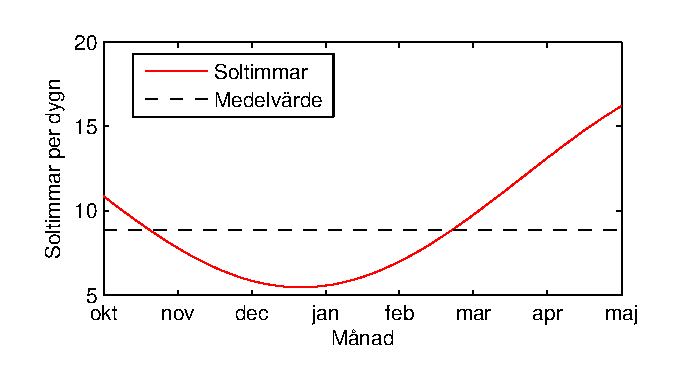
\includegraphics{images/sunhours.eps}
\caption{Antal timmar i ett dygn då solen är ovanför horisonten beräknat för månaderna under eldningsperioden.
Här är medelvärdet markerat med en streckad linje. Medelvärdet har beräknats vara
$\bar{\tau}=\unit[9,39]{~timmar~per~dygn}$.}
\label{fig:sunhours}
\end{figure}

\noindent
För att estimera hur mycket energi som det går att spara på att ta hänsyn till solen kommer arbetet
senare att behandla en decemberdag. Denna dag har sedan behandlats med antagandet att den är solig samt
med antagandet att den är molning. Vi benämner energiåtgången för den molniga dagen som $Q_H$ och
$Q_L$ som energiåtgången den soliga dagen. Värden på dessa kommer sedan att användas tillsammans med
ovanstående beräkningar för att estimera totala mängden energi som det går att spara. 

Från SMHIs väderstatistik går det att utläsa att $\unit[8]{\%}$ av eldningsperiodens timmar är soliga.\cite{SMHIdata}
Detta motsvarar då $\unit[1,92]{~soliga~timmar}$ i snitt per dygn. Härnäst betecknas andelen timmar som är molniga som
$p = 1,92/9,32 = \unit[20,45]{\%}$. Nu beräknas medelenergiåtgången per dygn $Q$ enligt

\begin{equation}
Q = pQ_H + (1-p)Q_L
\end{equation}

\noindent
Slutligen kan kvoten $Q/Q_H$ beräknas vilket ger ett uttryck för hur mycket energi det går att spara

\begin{equation}
\frac{Q}{Q_H} = \frac{pQ_H + (1-p)Q_L}{Q_H} = p+(1-p)\frac{Q_L}{Q_H}
\end{equation}

\subsection{Solinstrålning}
För att beräkna den totala effekt solstrålning tillför byggnaden via fönster behövs fönstrenas vinkelberoende g-värden, presenterat i avsnitt \ref{gvalue}, och för att bestämma detta värde ur \eqref{eq:radiationwindowstheory:gvalue} behöver parametern $z = \theta/90$ beräknas, där $\theta$ är vinkeln mellan solstrålingens riktning och fönstrets normal i grader. Detta kan göras genom att utgå från aktuellt datum och tid på dygnet.

En metod för att räkna ut solens position presenteras i \cite{walraven78} och en Matlabfunktion baserad på samma artikel kan ses i appendix \ref{app:sunposition}. Argumenten i denna funktion består av longitudinella och latitudinella koordinater för aktuella platsen samt datum och tidpunkt. För Walleriusgatan är koordinaterna ungefär $\unit[12]{^\circ}$ E respektive $\unit[58]{^\circ}$ N.

När azimuthala och altitudinella vinklarna, det vill säga $\beta$ respektive $\alpha$, relativt ett väderstreck respektive horisonten har beräknats relateras infallsvinkeln mot glaset, $\theta$, som

\begin{equation} 
\theta = \arccos{\left( \cos{\left(\beta - \gamma\right)}\cos{\left(\alpha\right)}\right)}
\end{equation}

där $\gamma$ är vinkeln mellan fönstrets normal och väderstrecket mot vilken azimuthala vinkeln anges. Detta görs med funktionen angletheta i appendix \ref{app:sunwindows}.

Med dessa samband tillgängliga kan effektflödet på grund av solstrålning genom fönster beräknas, vilket kan göras med funktionerna \textit{gvalue} samt \textit{effekt} från appendix \ref{app:sunwindows}. Nödvändiga argument för dessa funktioner är g-värdet vid vinkelrätt infallande strålning samt konstanterna p och q från \eqref{eq:gconstants}. % Repetera ekvationen?

För att ge ett exempel på hur effekten varierar med solintensiteten måste en approximativ funktion byggas upp som beskriver solens intensitet vid marknivå som funktion av vinkeln över horisonten. Om vi antar att intensiteten är $I_o = \unit[1370]{Wm^-2}$ utanför atmosfären kan detta beskrivas med ett exponentiellt samband, $I = I_oe^{-\mu x}$ där $\mu$ kallas för atmosfärens absorbtionskoefficient som sätts till $mu\approx \unit[4.6\cdot 10^{-5}]{m^{-1}}$ och x är atmosfärens tjocklek mellan betraktaren och solen, i meter. Atmosfären antas dessutom vara som en homogen heltäckande sfär runt jorden och ungefär $\unit[15]{km}$ tjock vertikalt uppåt överallt på jordens yta. x kan nu beskrivas med solens höjd över horisonten, och ges av

\begin{equation}
x = R\cos{90+\alpha} + \sqrt{\left(R\cos{90+\alpha}\right)^2 + \left( R+15\right)^2 - R^2}
\end{equation}

där $\alpha$ är vinkeln mellan horisonten och solen och $R\approx\unit[6,731\cdot 10^3]{m}$ betecknar jordens radie \cite{physicshandbook}. Detta följer från cosinussatsen. % Källa på siffran mu?

\subsubsection{Inverkan av skuggor, rummets interiör och dylikt}

Sambanden ovan gäller då all strålning som passerar rutan stannar i rummet. Svårigheter uppstår när exempelvis persienner används. Dessutom har ingen hänsyn tagits till det faktum att omkringliggande byggnader kommer att blockera den direkta solstrålningen vid vissa tidpunkter.

Hur mycket av solinstrålningen som blockeras av persienner och gardiner är oerhört svårt att räkna ut. För det första hyser den parametern ett vinkelberoende, det vill säga beroende på persiennens konfiguration, färg och vinkel kommer olika mycket att reflekteras tillbaka ut ur fönstret. För det andra måste hänsyn tas till mänskliga faktorer. Naturligtvis kommer vinkeln på persiennen att förändras vid godtyckliga tidpunkter. För att modellera sådana anordningar kan man enligt \cite{ASHRAE09} lägga till en vinkelberoende faktor, $0 \le R_{ref}\left( \theta \right) \le 1$, i \eqref{eq:totalsun} så att den slutliga formeln för solinstrålning genom fönster blir


\begin{equation}\label{eq:totalsunblinds}
Q = R_{ref}\left( \theta \right) \cdot g\left( \theta \right) \cdot A \cdot I_0 \cos{\theta} \unit[]{W}.
\end{equation}

Vid exempelberäkningarna i nästa avsnitt har dock ingen hänsyn tagits till denna koefficient, som satts konstant $R_{ref}$.

Effekten av skuggorna som orsakas av grannbyggnader i området kan också tas med i beräkningarna genom att mäta geometrin på omgivande byggnader, men detta är ett tidsödande moment och görs inte i denna rapport.

\subsection{Långvågsstrålning}\label{subsec:IRmethod}

Vid beräkning av energiflödet på grund av långvågig strålning antas att luften precis innanför fönstret håller konstant temperatur, $\unit[20]{^{\circ}C}$ och att de ''synliga'' ytorna utanför fönstret håller en temperatur motsvarande utomhustemperaturen, $T_{ute}$. Enligt beräkningen i avsnitt \ref{IR} kommer 75\% av den incidenta strålningen passera ett treglasfönster. Med detta i åtanke leder Stefan-Boltzmanns lag, \eqref{eq:boltzmanslag}, till, om det antas stråla som en svartkropp, att $q_{IR} = 0,75 \cdot \sigma \unit[\left( 293^4 - T_{ute}^4\right)]{Wm^{-2}}$. Den totala effekt som flödar ut på grund av svartkroppsstrålning blir då $\unit[q_{IR}\cdot A]{W}$, där $A$ är totala arean av fönsterglas på byggnaden.

\subsection{Övriga strålningseffekter}\label{subsec:otherradiation}

Då solen skiner kommer en viss andel direkt solstrålning att reflekteras från omgivande byggnader, växtlighet och dylikt för att sedan öka på intesiteten mot fönsterrutorna. Eftersom en andel av den direkt infallande solstrålningen genom fönsterrutorna även kommer att reflekteras mot rummens interiör och stråla ut igen har vi valt att inte ta hänsyn till dessa flöden, som beror starkt på omgivningens respektive interiörens utformning.


\section{Finita element av värmeledningsekvationen}

I detta avsnitt behandlas finita elementlösningen av värmeledningsekvationen.
Det är från avsnitt \ref{sec:heatconduction} givet att differentialekvationen
enligt ekvation \eqref{eq:femheateq} beskriver värmeflöde i ett material.

\begin{equation}
\label{eq:femheateq}
c_p\rho\frac{\partial T}{\partial t} = \nabla\cdot(k\nabla T)
\end{equation}

\noindent
För att finna en lösning integreras värmeledningsekvationen
multiplicerat med en $L^2$ integrabel testfunktion $\phi(\mathbf{r})$ över hela
definitionsmängden $\Omega$ vars rand benämns $\Gamma$.
Detta kan ses i ekvation \eqref{eq:femheatweak}.
Nu söks en funktion $T(\mathbf{r},t)$ som satisfierar nyss nämnda uttryck för
alla $L^2$ integrabla testfunktioner $\phi(\mathbf{r})$.

\begin{equation}
\label{eq:femheatweak}
\int_\Omega \left(c_p\rho\frac{\partial T}{\partial t} -
\nabla\cdot(k\nabla T)\right)\phi(\mathbf{r})d\Omega = 0
\end{equation}

\noindent
För att förenkla fortsatta beräkningar behövers det genomföras några
omskrivningar av uttrycket. Divergensteoremet används först för att 
eliminera divergensen i värmeledningsekvationens högerled. Detta ger då
ekvation \eqref{eq:femheatweakfull}. Här är $\mathbf{n}$ normalen till randen.

\begin{equation}
\label{eq:femheatweakfull}
\int_\Omega c_p\rho\frac{\partial T}{\partial t}\phi(\mathbf{r}) +
k\nabla T\nabla\phi(\mathbf{r}) d\Omega =
\int_\Gamma k\mathbf{n}\cdot\nabla Td\Gamma
\end{equation}

\noindent
Härnäst skall galerkinformuleringen skissas. Detta genomförs
genom att temperaturen $T$ samt tidsderivatan av temperaturen $\dot{T}$
enligt ekvationerna \eqref{eq:femheatt} och \eqref{eq:femheattdot}.

\begin{align}
\label{eq:femheatt}
T(\mathbf{r}) & \approx \sum_n T_n\phi(\mathbf{r}) \\
\label{eq:femheattdot}
\dot{T}(\mathbf{r}) & \approx \sum_n \dot{T}_n\phi(\mathbf{r})
\end{align}

\noindent
Ansatsen ovan stoppas härnäst in i den svaga formuleringen i ekvation
\eqref{eq:femheatweakfull} vilket ger ekvation \eqref{eq:femheatgalerkin}.
För att kunna lösa problemet för definitionsmängder som består av olika
homogena material väljs testfunktionen $\phi$ så att den försvinner vid
alla andra material än ett och värmeledningskonstanten kan då benämnas $k_n$.
Ekvationssystemet kan sedan skrivas i matrisform vilket kan ses i ekvation
\eqref{eq:femheatmatrix}. Här är $M$ massmatrisen, $A$ är stelhetsmatrisen och
$f$ är belastningsvektorn.

\begin{align}
\label{eq:femheatgalerkin}
\sum_n \dot{T}_n \int_\Omega c_p\rho\phi_i(\mathbf{r})
\phi_n(\mathbf{r})d\Omega
& + \sum_n T_n \int_\Omega k_n \nabla\phi_n(\mathbf{r})\nabla\phi_n(\mathbf{r})
d\Omega \\
&= \int_\Gamma k_i\phi_i\mathbf{n}\cdot\nabla Td\Gamma \Leftrightarrow
\nonumber
\end{align}

\begin{equation}
\label{eq:femheatmatrix}
M\dot{T} + AT = f \Rightarrow
\end{equation}

\begin{equation}
\label{eq:femheatmatrix2}
\dot{T} + M^{-1}AT = M^{-1}f
\end{equation}

\noindent
Som kan ses så är ovanstående uttryck ett system av kopplade ordinära
differentialekvationer vars lösning är trivial med hjälp av egenvärdesuppdelning.
Vektorerna $\{v\}^n_{i=1}$ definieras som egenvektorerna av
$M^{-1}A$ och $\lambda_i$ definieras som egenvärdena till samma matris.
Systemets homogena lösning kan då skrivas som ekvation
\eqref{eq:femheathom}.\cite{lay06}

\begin{equation}
\label{eq:femheathom}
T_h(t) = \sum_n = c_n\mathbf{v}_ne^{-\lambda_nt}
\end{equation}

\noindent
Då ekvationen är inhomogen så återstår det att lösa systemets
partikulärlösning. Då inhomogeniteten är konstant så kan lämpligen
en konstant ansättas som partikulärlösning. Detta ger att
$T_p(t) = D$. Insättning i differentialekvationen ger
ekvation \eqref{eq:femheatinstopp} vilket gör att vi kan bestämma
$D$ genom ekvation \eqref{eq:femheatinstopp2}.

\begin{align}
\label{eq:femheatinstopp}
M^{-1}AD &= M^{-1}b \Rightarrow\\
\label{eq:femheatinstopp2}
D &= A^{-1}b
\end{align}

\noindent
Nu kan den fullständiga lösningen skissas som $T = T_h + T_p$ och om
tiden sätts till noll så kan konstanterna $c_n$ bestämmas genom
att $T$ sätts till problemets begynnelsevärden. För ett problem som
saknar tidsberoende eller som har nått en jämviktspunkt måste
tiden vara oändlig och de termer som innehar exponenter blir noll.
Detta innebär att partikulärlösningen $T_p$ är den tidsoberoende lösningen
till problemet. Detta kan enkelt verifieras genom att sätta $\dot{T} = 0$.
Problemet som återstår är då $AT = b$ vars lösning är $T_p$.

\section{Värmeflöde genom vägg}

För att jämföra energiförluster genom en vägg med isolering och utan isolering används
den tidigare beskrivna finita elementmetoden för värmeledningsekvationen i en dimension. Här approximeras
väggen som oändligt lång för simplicitet i beräkningarna. För alla beräkningar så har ett tidssteg
på $\Delta t = \unit[500]{s}$ använts med semidiskret MOL.

I detta försök antags det att en perfekt värmeanläggning
existerar så att temperaturen inomhus hålls till konstanta $\unit[20]{^\circ C}$. Efter detta specificeras energiflödet
från utsidan av väggen genom vilka energiflöden som strömmar till väggen. Dessa är svartkroppsstrålning, solinstrålning
samt konvektion. Beräkningarna är sedan genomförda med solinstrålningsdata från en molning nyårafton,
en solig aprildag samt en molning aprildag.\emph{\color{red} Lägg till referenser/information om solinstrålning och svartkroppsstrålning}.
Konvektionsparametern är sedan satt till $h=\unit[6,19]{Wm^{-2}K^{-1}}$ för aprildagen vilket motsvarar en helt vindstilla aprildag.
För decemberdagen sattes konvektionsparametern till $h=\unit{35}{Wm^{-2}K^{-1}}$ vilket motsvarar en
\emph{ \color{red} hur blåsig decemberdag?}.
Under aprildagen varierade temperaturen linjärt från $T=\unit[6]{^\circ C}$ klockan 06:00 och $T=\unit[9]{^\circ C}$ 16:00.
Samma värden för decemberdagen är $T = \unit[-11]{^\circ C}$ 06:00 respektive $T=\unit[-5]{^\circ C}$ 16:00.

Problemet har sedan satts upp för två olika väggar. Först en som enbart innehåller $\unit[5]{dm}$ tegel med
en värmeledningsförmåga på $k_{tegel} = \unit[0.6]{Wm^{-1}K^{-1}}$ och volymetrisk värmekapacitet på
$c_{p tegel}\rho_{tegel} = \unit[1,153846]{MJ kg^{-1}}$. Den andra väggen har först samma tegellager sedan
har den tilläggsisolerats på utsidan med $\unit[1]{dm}$ mineralull. Denna mineralull har värmeledningsförmåga på
$k = \unit[5,2\cdot 10^{-7}]{Wm^{-1}K^{-1}}$ och volymetrisk värmekapacitet på
$c_{p isolering}\rho_{isolering} = \unit[58,8]{kJ kg^{-1}}$.
\emph{\color{red} Källor på naturkonstanter}

Under experimentens gång så har ett godtyckligt initialvärde valts för att sedan vänta tills
lösningen stabiliserat sig för att då urläsa energiåtgången. Derivatan på insidan har slutligen beräknats
och använts för att beräkna kyleffekten genom fouriers värmelag.

För att studera hur de olika väggarna beter sig vid ett stegsvar har ett sådant tillverkats. Experimentet
har startats med att väggarna varit i jämvikt med en utomhustemperatur på $T = \unit[0]{^\circ C}$ för att
sedan stiga till $T = \unit[10]{^\circ C}$ vid tiden $t=0$. Konvektionsparametern är här satt till
$h = \unit[25]{W m^{-1}K^{-1}}$ \emph{\color{red} vilket motsvarar ?????}. Slutligen så kunde väggarnas
tröghet studeras genom att den momentana kyleffekten beräknades för varje tidssteg. 

\section{Värmeflöde genom grunden}

\emph{\color{red} Randvillkor? $h=15,5$. Svartkroppsstrålning. Sol enligt graf nedan.}

\begin{figure}
\centering
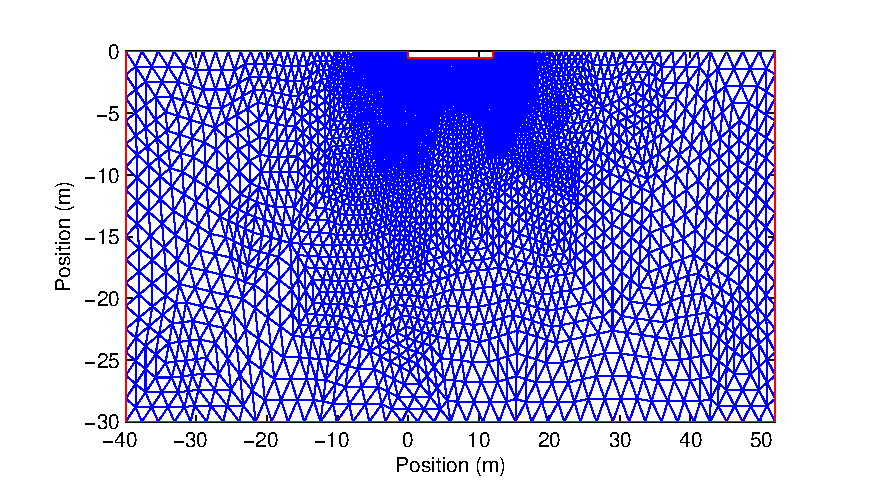
\includegraphics{images/trifoundation.eps}
\caption{Definitionsmängd samt triangulering berget under grunden.}
\end{figure}


\begin{figure}
\centering
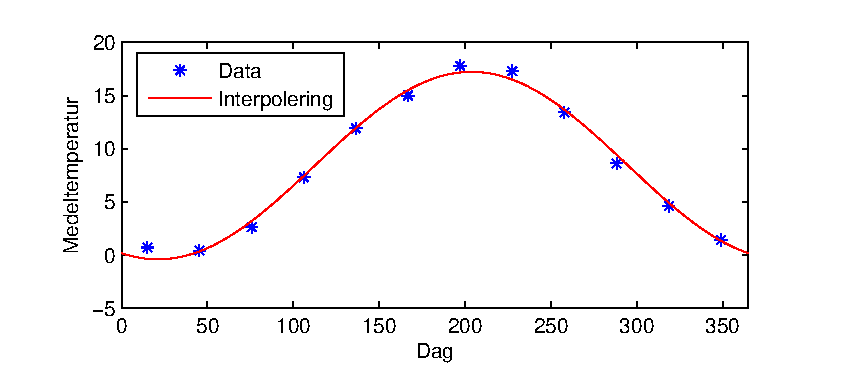
\includegraphics{images/meantemperature.eps}
\caption{
Medeltemperaturen för göteborg de senaste 20 åren. Punkterna är data tagna från Miljöförvaltningen och linjen är minstakvadratanpassningen som senare använts för att beräkna energiflöden.}
\end{figure}

%Miljöförvaltningen
%http://www4.goteborg.se/prod%5Csk%5Cstatistik%5CstatistikR5.nsf/0/3F002A395ED39AC8C1256D3B00393D0E/$File/3.01.pdf

\subsection{Finita element av inkompressibel fluid}

För att lösa Navier-Stokes ekvationer kan lämpligen en datormodell användas.
Här består denna modell av ett system uppsatt med Galerkins metod.
I denna lösning så begränsar vi dock oss till att enbart behandla statiska flöden
vilket genomförs genom att sätta alla tidsderivator till noll.

För att hantera trycket i \eqref{eq:convection:continuity}-\eqref{eq:convection:energy} används den tidigare nämnda Boussinesq approximation
samt penalty metoden för att göra hastighetsvektorn källfri och uppfylla
kontinuitetsekvationen. Det finns således inget direkt behov av att räkna ut trycket.
Vid användning av många sorters elementtyper som inte uppfyller Babuska-Brezzikriteriet
är detta dessutom nödvändigt då det annars kan bildas oönskade trycknoder. 
En annan möjlighet är att välja divergensfria element. \cite{babuska1973}\cite{segal2011}

Genom penaltymetoden beskrives här trycket som $p$ enligt ekvation
\eqref{eq:femconvection:penalty}. Här är $p_s$ någon form av idealt statiskt
tryck som är önskat. Detta tryck följer Boussinesq approximation. Med dessa
idealiseringar kan differentialekvationerna sättas upp igen. \cite{heinrich88}\cite{taylor79}
Som kan ses så leder den godtyckliga penaltyparametern $\lambda$ till att justera trycket
om hastighetsfältets divergens ej är identiskt noll. I viss litteratur anges 
det att penaltyparametern skall vara i storleksordningen $10^7$ men att den
är väldigt applikationsberoende. En för liten vald penaltyparameter leder till att
trycket inte elimineras. Andra problem uppstår vid en för stor parameter. Ekvationssystemet
kan bli svårlöst och få stabilitetsproblem när parametern blir
för stor i jämförelse med de andra delarna i differentialekvationen.\cite{reddy93}\cite{roy05}\cite{basak04}\cite{segal2011}

\begin{equation}
\label{eq:femconvection:penalty}
p = p_s - \lambda\nabla\cdot\mathbf{v}
\end{equation}

\noindent
Fortsatt skall trycket deriveras med avseende på de rumsliga variablerna vilket möjliggör
att eliminera trycket från differentialekvationerna. Dessa deriveringar kan ses i ekvation
\eqref{eq:femconvection:partx} samt \eqref{eq:femconvection:partz}. Notera att det statiska trycket
$p_s$ ej beror på $x$ vilket resulterar i att derivatan är noll.

\begin{equation}
\label{eq:femconvection:partx}
\frac{\partial p}{\partial x} = \frac{\partial p_s}{\partial x} -
\frac{\partial}{\partial x} \lambda\nabla\cdot\mathbf{v} = -
\frac{\partial}{\partial x} \lambda\nabla\cdot\mathbf{v}
\end{equation}

\begin{equation}
\label{eq:femconvection:partz}
\frac{\partial p}{\partial z} = \frac{\partial p_s}{\partial z} -
\frac{\partial}{\partial z} \lambda\nabla\cdot\mathbf{v} =
-g\rho_0 - \frac{\partial}{\partial z} \lambda\nabla\cdot\mathbf{v}
\end{equation}

\noindent
Detta förs in i momentekvationerna vilket ger ekvationerna \eqref{eq:femconvection:u} -
\eqref{eq:femconvection:T}. Här är det ekvationssystem som syftar att lösas.

\begin{equation}
\label{eq:femconvection:u}
\mathbf{v}\cdot\nabla u =
\frac{\lambda}{\rho_0}\nabla\cdot\mathbf{v} +
\nu\Delta u
\end{equation}

\begin{equation}
\label{eq:femconvection:w}
\mathbf{v}\cdot\nabla w =
\frac{\lambda}{\rho_0}\nabla\cdot\mathbf{v} + \nu\Delta w +g\beta(T-T_0)
\end{equation}

\begin{equation}
\label{eq:femconvection:T}
\mathbf{v}\cdot\nabla T = \alpha\Delta T
\end{equation}

\subsubsection{Svag formulering}

En finita elementlösning med Galerkins metod kräver att problemet reduceras till
ett ekvivalent variationsproblem. Här söks $T\in\Phi$, $u\in\Phi$ och
$w\in\Phi$ som uppfyller ekvation \eqref{eq:femconvection:variation}. Här
betecknar brackets skalärprodukt, $\mathbf{L}$ är differentialoperatorn
som betecknar systemet av differentialekvationer som $\mathbf{L}(T,u,w) = 0$.
$\Phi$ är rummet av alla testfunktioner $\phi$ som är kontinuerliga i
definitionsmängden $\Omega$ samt vars derivator är bitvis kontinuerliga på randen
$/Gamma$. De måste även vara $L^2$ integrabla.

\begin{equation*}
\label{eq:femconvection:variation}
\langle \mathbf{L}(T,u,w), \phi \rangle = 0\mbox{,  } \forall \phi \in \Phi
\end{equation*}


\subsection{Datorsimulering av ofrivillig ventilation}


